\documentclass[a4paper,12pt]{article}

\usepackage[utf8]{inputenc}
\usepackage[T1]{polski}
\usepackage{helvet}
\usepackage{graphicx}
\usepackage{color}
\usepackage{xcolor}
\usepackage{geometry}
\usepackage{register}
\usepackage{listings}
\usepackage{caption}
\usepackage{makeidx}
\usepackage{longtable}
\usepackage{multirow}
\usepackage{wrapfig}


\geometry{hmargin={2cm, 2cm}, height=10.0in}
\DeclareCaptionFont{white}{\color{white}}
\DeclareCaptionFormat{listing}{\colorbox{gray}{\parbox{\textwidth}{#1#2#3}}}
\captionsetup[lstlisting]{format=listing,labelfont=white,textfont=white}
\lstset{ %
language=Octave,                % choose the language of the code
basicstyle=\footnotesize,       % the size of the fonts that are used for the code
numbers=left,                   % where to put the line-numbers
numberstyle=\footnotesize,      % the size of the fonts that are used for the line-numbers
stepnumber=1,                   % the step between two line-numbers. If it's 1 each line 
                                % will be numbered
numbersep=5pt,                  % how far the line-numbers are from the code
backgroundcolor=\color{white},  % choose the background color. You must add \usepackage{color}
showspaces=false,               % show spaces adding particular underscores
showstringspaces=false,         % underline spaces within strings
showtabs=false,                 % show tabs within strings adding particular underscores
frame=single,	                % adds a frame around the code
tabsize=2,	                % sets default tabsize to 2 spaces
%captionpos=b,                   % sets the caption-position to bottom
breaklines=true,                % sets automatic line breaking
breakatwhitespace=false,        % sets if automatic breaks should only happen at whitespace
title=\lstname,                 % show the filename of files included with \lstinputlisting;
                                % also try caption instead of title
escapeinside={\%*}{*)},         % if you want to add a comment within your code
morekeywords={*,...}            % if you want to add more keywords to the set
}

\lstloadlanguages{ Verilog }

\makeindex

\begin{document}

% =====  STRONA TYTULOWA PRACY MAGISTERSKIEJKIEJ ====
% ostatnia modyfikacja: 2009/07/01, K. Malarz

\thispagestyle{empty}
%% ------------------------ NAGLOWEK STRONY ---------------------------------
\begin{figure}
\vspace{-13cm}
\hspace{-4cm}

\includegraphics[height=29.3cm]{grafika/agh_nzw_a_pl_1w_wbr_cmyk.pdf}\\
\vspace{-13.9cm}
\end{figure}
\rule{26mm}{0pt}
{\large\textsf{Wydział Fizyki i Informatyki Stosowanej}}\\
\rule{\textwidth}{3pt}\\
\rule[2ex]
{\textwidth}{1pt}\\
\vspace{7ex}
\begin{center}
{\LARGE \bf \textsf{Praca magisterska}}\\
\vspace{13ex}
% --------------------------- IMIE I NAZWISKO -------------------------------
{\bf\Large\textsf{Krystian Wojtas}}\\
\vspace{3ex}
{\sf \small kierunek studiów:} {\bf\small\textsf{informatyka stosowana}}\\
\vspace{1.5ex}
{\sf \small kierunek dyplomowania:} {\bf\small\textsf{metody numeryczne}}\\
\vspace{10ex}
%% ------------------------ TYTUL PRACY --------------------------------------
{\bf \huge \textsf{Oprogramowanie sprzętu laboratoryjnego dedykowanego dla przedmiotu "Projektowanie Systemów Cyfrowych"}}\\
\vspace{6ex}
%% ------------------------ OPIEKUN PRACY ------------------------------------
{\Large Opiekun: \bf \textsf{dr inż. Krzysztof Świentek}}\\
\vspace{28ex}
{\large \bf \textsf{Kraków, czerwiec 2012}}
\end{center}
%% =====  STRONA TYTUŁOWA PRACY MAGISTERSKIEJKIEJ ====

\newpage

%% =====  TYŁ STRONY TYTUŁOWEJ PRACY MAGISTERSKIEJKIEJ ====
{\sf Oświadczam, świadomy(-a) odpowiedzialności karnej za poświadczenie nieprawdy, że niniejszą pracę dyplomową wykonałem(-am) osobiście i samodzielnie i  nie korzystałem(-am) ze źródeł innych niż wymienione w pracy.}

\vspace{14ex}

\begin{center}
\begin{tabular}{lr}
~~~~~~~~~~~~~~~~~~~~~~~~~~~~~~~~~~~~~~~~~~~~~~~~~~~~~~~~~~~~~~~~~ &
................................................................. \\
~ & {\sf (czytelny podpis)}\\
\end{tabular}
\end{center}

%% =====  TYL STRONY TYTULOWEJ PRACY MAGISTERSKIEJKIEJ ====

\newpage
\rightline{Kraków, czerwiec 2012}
\begin{center}
{\bf Tematyka pracy magisterskiej i praktyki dyplomowej
Jana Nowaka,
studenta V roku studiów kierunku fizyka techniczna, specjalności fizyka komputerowa}\\
\end{center}

Temat pracy magisterskiej:
{\bf Tu wpisz temat pracy magisterskiej Temat pracy magisterskiej Temat pracy magisterskiej}\\

\begin{tabular}{rl}

Opiekun pracy:                  & prof. dr hab. Śmaki Owaki\\
Recenzenci pracy:               & dr hab. inż. Owaki Śmaki\\
Miejsce praktyki dyplomowej:    & WFiIS AGH, Kraków\\
\end{tabular}

\begin{center}
{\bf Program pracy magisterskiej i praktyki dyplomowej}
\end{center}

\begin{enumerate}
\item Omówienie realizacji pracy magisterskiej z opiekunem.
\item Zebranie i opracowanie literatury dotyczącej tematu pracy.
\item Praktyka dyplomowa:
\begin{itemize}
\item zapoznanie się z ideą...,
\item uczestnictwo w eksperymentach/przygotwanie oprogramowania...,
\item dyskusja i analiza wyników...
\item sporządzenie sprawozdania z praktyki.
\end{itemize}
\item Kontynuacja obliczeń związanych z tematem pracy magisterskiej.
\item Zebranie i opracowanie wyników obliczeń.
\item Analiza wyników obliczeń numerycznych, ich omówienie i zatwierdzenie przez opiekuna.
\item Opracowanie redakcyjne pracy.
\end{enumerate}


\noindent
Termin oddania w dziekanacie: ?? czerwca 20??\\[1cm]

\begin{center}
\begin{tabular}{lcr}
.............................................................. & ~~~ &
.............................................................. \\
(podpis kierownika katedry) & & (podpis opiekuna) \\
\end{tabular}
\end{center}

\newpage
\noindent
Na kolejnych dwóch stronach proszę dołączyć kolejno recenzje pracy popełnione przez Opiekuna oraz Recenzenta (wydrukowane z systemu MISIO i podpisane przez odpowiednio Opiekuna i Recenzenta pracy). Papierową wersję pracy (zawierającą podpisane recenzje) proszę złożyć w dziekanacie celem rejestracji co najmniej na tydzień przed planowaną obroną.

\newpage
\noindent
Na kolejnych dwóch stronach proszę dołączyć kolejno recenzje pracy popełnione przez Opiekuna oraz Recenzenta (wydrukowane z systemu MISIO i podpisane przez odpowiednio Opiekuna i Recenzenta pracy). Papierową wersję pracy (zawierającą podpisane recenzje) proszę złożyć w dziekanacie celem rejestracji co najmniej na tydzień przed planowaną obroną.

\newpage
\section{Cel pracy}

\begin{figure}[htb]
   \centering
   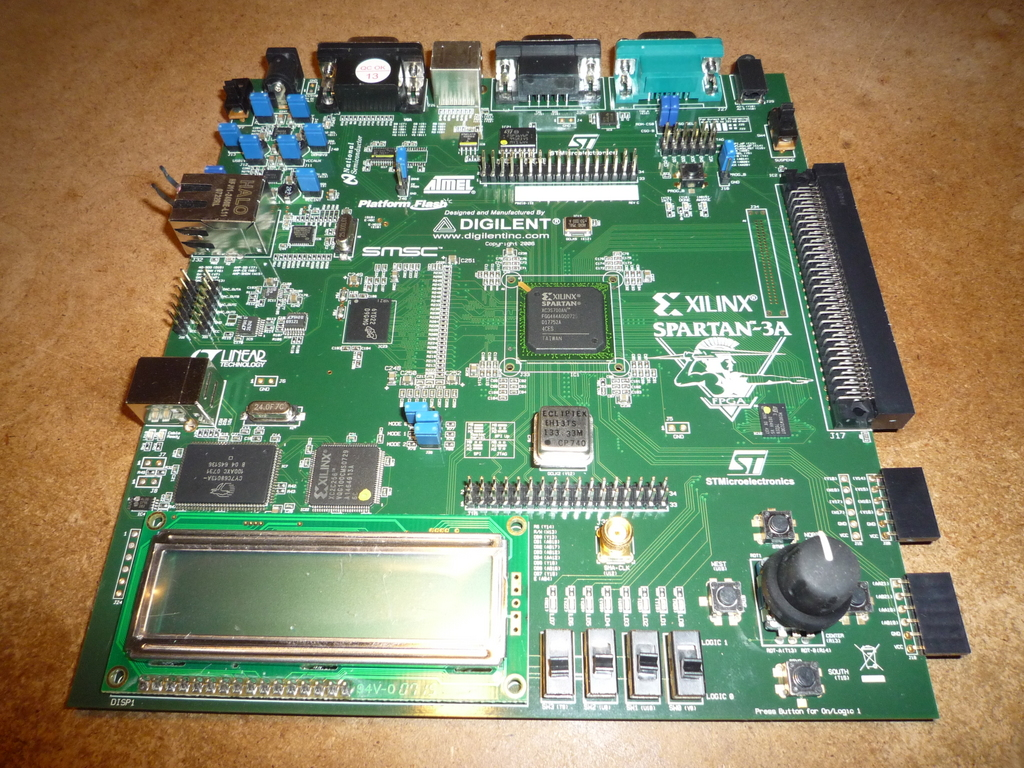
\includegraphics{grafika/spartan3an.jpg}
   \caption{Xilnix Spartan-3AN Starter Kit}
\end{figure}

Celem pracy jest oprogramowanie za pomocą języka opisu sprzętu (Verliog) układów używanych podczas zajęć laboratoryjnych z Projektowanie Systemów Cyfrowych. Praca polegałaby na przygotowaniu zestawu syntezowalnych bloków HDL do wszystkich elementów płytki „Xilnix Spartan-3AN Starter Kit” (www.xilinx.com/products/devkits/HW-SPAR3AN-SK-UNI-G.htm). Dodatkowo należy opracować modele behawioralne służące do testowania poprawności kodu (poszczególnych modułów sprzętu) tworzonego przez studentów podczas zajęć. Podsumowaniem całości ma być projekt kompleksowo demonstrujący możliwości wyżej wspomnianego sprzętu.  

Utworzone moduły behawioralne muszą (wiernie) odzwierciedlać zachowania układów występujących na płytce.
Znajdą wtedy zastosowanie w uruchamianych symulacjach przebiegów czasowych danej konfiguracji układu programowalnego FPGA. Dzięki nim możliwe będzie stwierdzenie czy dla zsyntetyzowanej konfiguracji stany linii FPGA prowadzące do konkretnego układu płytki przebiegają poprawnie i czy zachodzi pożądana komunikacja poprzez generowanie przez te moduły stosownych komunikatów. W ten sposób studenci będą mogli testować poprawność działania utworzonej przez siebie konfiguracji bez fizycznego dosępu do sprzętu.  
%zsyntetysowanej/wysyntetyzowanej


\newpage
\section{DAC}
Zadaniem konwertera cyfrowo-analogowego jest przetwarzanie przekazanych mu kolejnych liczb binarnych na ich analogowe odpowiedniki realizowane jako wartość napięcia na jego pinie wyjściowym w zakresie napięcia maksymalnego $V_{ref}$.

Obsługiwany przez przetwornik zakres liczb binarnych jest dokładnością przetwornika. Występujący na płytce układ scalony LTC2624 ma zatopione 4 przetworniki DAC o dokładności 12-bitowej. Wszystkie przetworniki domyślnie mają wartość napięcia maksymalnego $V_{ref} = 3.3V$, jednak dla dwóch z nich wartość tą można indywidualnie ustawić komunikując się z układem wzmacniaczy zawartych w kostce LP3906. Wartości napięć wyjściowych podaje wzór
$$V_{out} = \frac{D[11:0]}{4096}  V_{ref}$$

\subsection{Komunikacja}

\subsubsection{SPI}
Układ LTC2624 zaimplementowaną ma logikę komunikacji w standardzie magistrali Serial Peripheral Interface.

\begin{figure}[htb]
   \centering
   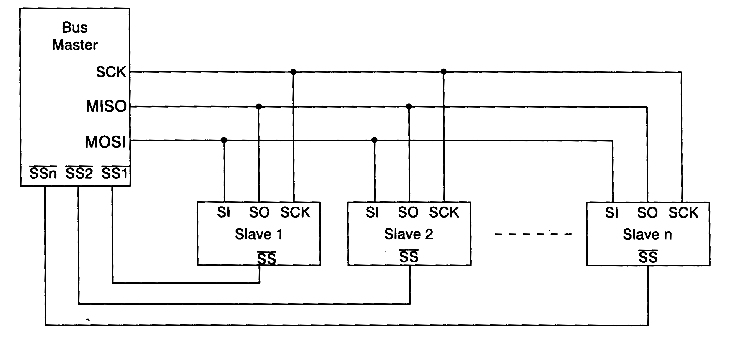
\includegraphics[width=15cm]{grafika/spi.jpg}
   \caption{SPI}
\end{figure}

Na magistrali występuje jeden układ nadrzędny - Master oraz co najmniej jeden Slave. 
Master generuje zegar na linii SCK. 
Master wysyła dane do Slavów szeregowo linią MOSI, Slavy odsyłają dane linią MISO. Transmisja jest fullduplexowana - przesył w obu kierunkach poszczególnych bitów następuje równocześnie w takt zegara.
Między układami współdzielone są linie zegara oraz danych. Odseparowane natomiast są linie CS poszczególnych slavów - wywołanie niskiego potencjału przez mastera aktywuje danego slava do uczestnictwa w wymianie danych.


\newpage
\subsubsection{Połączenia}

\begin{figure}[htb]
   \centering
   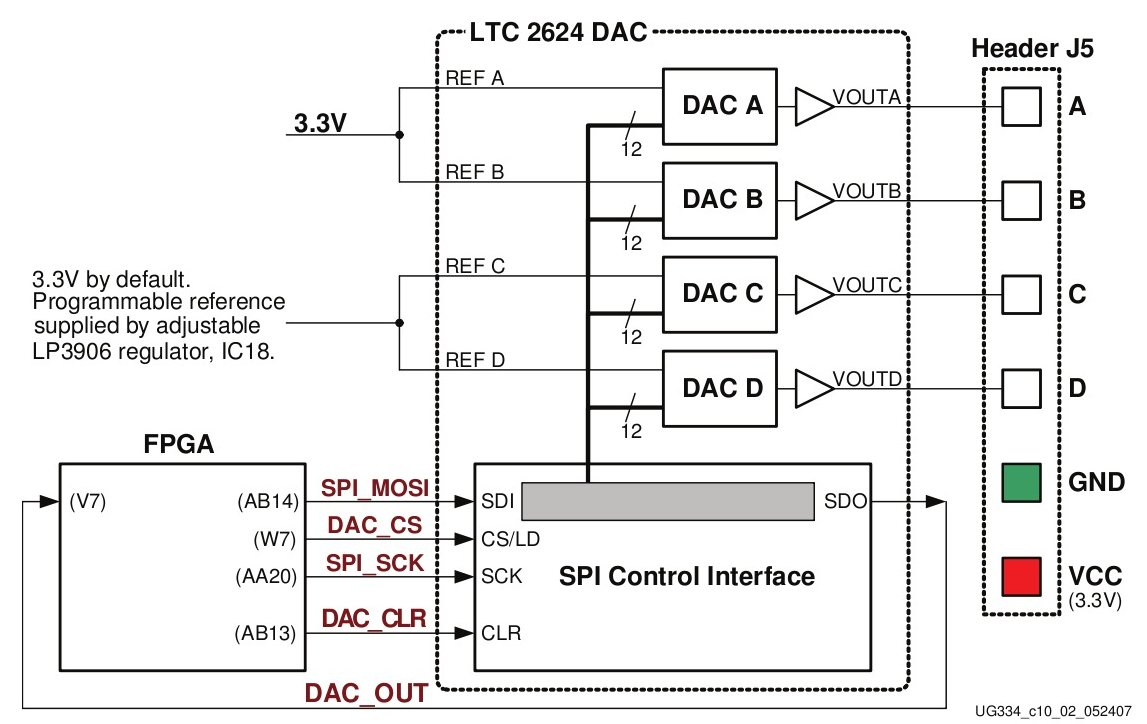
\includegraphics[width=15cm]{grafika/dac.jpg}
   \caption{Schemat polaczen ukladow LTC2624 i FPGA}
\end{figure}

Przed pierwszym użyciem należy układ zresetować chwilowo obniżając stan linii DAC\_CLR.

Na linie SPI\_SCK należy podać zegar o częstotliwości nie przekraczającej 50Mhz. Obniżając stan linii DAC\_CS rozpoczynamy komunikację z układem. Wtedy w takt zegara przesyłamy szeregowo do niego kolejne bity danych linią SPI\_MOSI. LTC2624 ładuje kolejne przesyłane bity do swojego rejestru przesuwnego na narastającym zboczu zegara oraz zwraca swoją poprzednią zawartość linią DAC\_OUT na opadającym zboczu. Natychmiast po wysłaniu kompletu danych należy koniecznie podnieść stan linii DAC\_CS zakańczając transmisję.

\begin{figure}[htb]
   \centering
   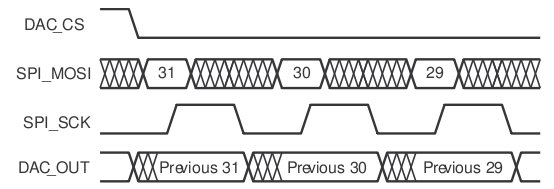
\includegraphics[width=15cm]{grafika/dac-waveform.jpg}
   \caption{Wykres stanow linii}
\end{figure}


\newpage
\subsubsection{Protokół komunikacji}

\begin{figure}[htb]
  \centering
	\begin{register}{H}{Przesylana ramka}{a}
	\label{dacprotocol}%
	\regfield{Nieistotne}{8}{24}{10000000}%
	\regfield{Komenda}{4}{20}{1100}%
	\regfield{Adres}{4}{16}{1111}%
	\regfield{Wartosc}{12}{4}{100000000000}%
	\regfield{Nieistotne}{4}{0}{0001}%
	\end{register}
\end{figure}

Dane przesyłane do układu LTC2624 są 32-bitową ramką uwidocznioną powyższym polem bitowym. Bity wysyła się kolejno zaczynając od najstarszego. Transmisja zaczyna się ośmioma nic nie znaczącymi bitami. Po nich wysyłane jest 4-bitowe pole komendy - typowo o wartości $0011$, co oznacza natychmiastowe wystawienie zadanej wartości napięcia. Następnie podawany jest adres konwertera według poniższej tabeli

\begin{figure}[htb]
  \centering
	\begin{tabular}{|c|c|c|c|l|}
	  \multicolumn{1}{r}{19}&\multicolumn{1}{r}{}&\multicolumn{1}{r}{}&\multicolumn{1}{r}{16}&\multicolumn{1}{l}{Adres}\\
		\hline 
		0&0&0&0 & DAC A\\
		\hline
		0&0&0&1 & DAC B\\
		\hline
		0&0&1&0 & DAC C\\
		\hline
		0&0&1&1 & DAC D\\
		\hline
		1&1&1&1 & Wszystkie\\
		\hline
	\end{tabular} 
\end{figure}

Trzecie pole jest 12-bitową wartością binarną odpowiadającą wystawianemu napięciu. Ramka kończy się 4 nieistotnymi bitami. W przykładzie na wszystkich konwerterach pojawiłaby się połowa z ustawionych zakresów napięć.


%\newpage
\subsection{Moduł behawioralny}
Wykonana została wzorcowa konfiguracja FPGA poprawnie ustawiająca DAC-i. Przedstawiona symulacja pokazuje wykres przebiegów czasowych linii prowadzących do układu DAC. Układ taktowany jest zegarem 50Mhz pochodzącym z kwarcu dostępnego na płytce. Przesyłana ramka jest przykładem z poprzedniego rozdziału - połowa zakresów napięć wystawiana na wszystkich dac-ach. Pola z bitami nieistonymi są tak ustawione aby pojedynczymi, skrajnymi pikami pokazywały początek i koniec ramki.

\begin{figure}[htb]
   \centering
   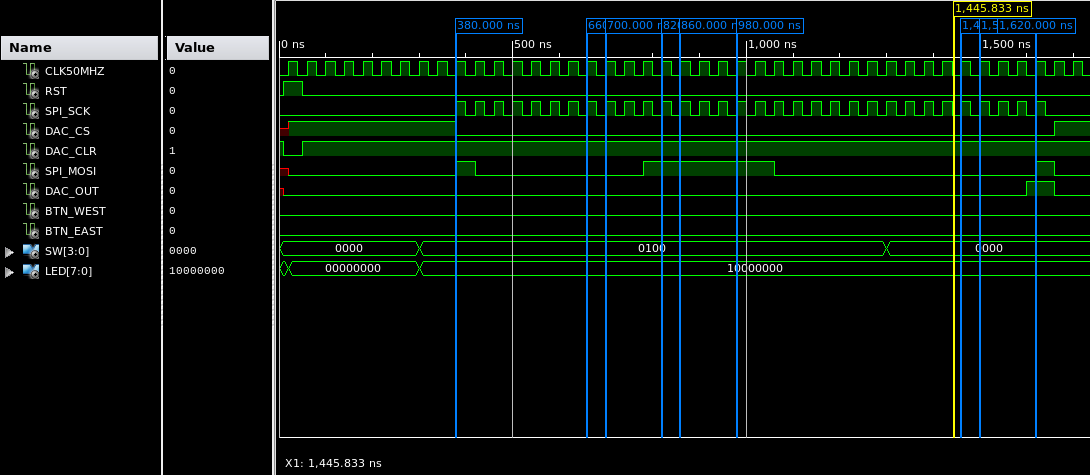
\includegraphics[width=13cm]{grafika/toptest-fastdac-110.png}
\end{figure}


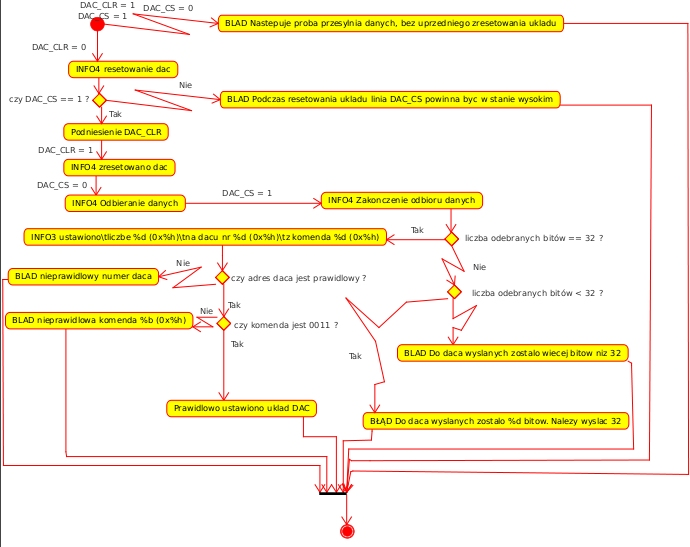
\includegraphics[width=15cm]{grafika/dac-uml.jpg}

\lstinputlisting[label=dac,caption=dacLTC2624behav.v]{zrodla/dacLTC2624-behav.v}

\linespread{1.3}
\selectfont

\end{document}

